\documentclass[
    11pt,
    spanish,
	a4paper
]{article}
\usepackage[utf8]{inputenc}
\usepackage[spanish]{babel}
\usepackage{graphicx}
\usepackage{authoraftertitle}
\usepackage{float}
\usepackage{caption}
\usepackage{verbatim}
\usepackage{listings}
\captionsetup[table]{labelformat=empty}

\def\doctype{Trabajo práctico}
\title{Transformada de Fourier}
\author{Gonzalo Nahuel Vaca}

\begin{document}

\makeatletter
\begin{titlepage}
	\begin{center}
		\vspace*{1cm}
		
		\Huge
		\textbf{\doctype}
		\vspace{0.5cm}
    
		\LARGE
		\@title
		\vspace{0.5cm}
    
		\textbf{Procesamiento Digital de Señales (fundamentos)}
		
		\vspace{1.5cm}
		
		\textbf{\@author}

		\vspace{1.5cm}

		
\includegraphics[width=0.8\textwidth]{img/logoFIUBA.pdf}
		
		\vfill
		Maestría en Sistemas Embebidos\\
		Universidad de Buenos Aires\\
		Argentina\\
		\today
	\end{center}
\end{titlepage}
\makeatother
\newpage

\section{Resolución}

\begin{lstlisting}[
    basicstyle=\tiny, %or \small or \footnotesize etc.
    ]
import numpy as np
import matplotlib.pyplot as plt


if __name__ == "__main__":
    fig = plt.figure(1)
    fs = 1
    sig_f_in = np.load("./fft_hjs.npy")[::1]
    sig_f_shifted = np.fft.fftshift(sig_f_in)
    N = len(sig_f_in)
    exclude_points = 0
    Nmod = N - exclude_points
    inf_lim = int(exclude_points / 2)
    sup_lim = int(N - exclude_points / 2)
    n = np.arange(-N / 2, N / 2, 1) / fs
    sig_f_trunc = np.fft.ifftshift(sig_f_shifted[inf_lim:sup_lim])
    fftAxe = fig.add_subplot(2, 2, 1)
    fftAxe.set_title("Espectro en frecuencia")
    fftAxe.grid(True)
    fftAxe.plot(n, np.real(sig_f_shifted), "b-")
    fftAxe.plot(n, np.imag(sig_f_shifted), "r-")
    fftAxe.fill_between(
        [(-N // 2 + inf_lim), (sup_lim - N / 2)],
        200,
        -200,
        facecolor="yellow",
        alpha=0.2,
    )
    n = np.arange(0, Nmod, 1) / fs
    sig_t = np.fft.ifft(sig_f_trunc)
    ifftAxe = fig.add_subplot(2, 2, 2)
    ifftAxe.set_title("Senal en tiempo")
    ifftAxe.grid(True)
    ifftAxe.plot(n, np.real(sig_t), "b-")
    ifftAxe.plot(n, np.imag(sig_t), "r-")
    ifft2d = fig.add_subplot(2, 2, 3)
    ifft2d.set_title("IDFT en 2D")
    ifft2d.grid(True)
    ifft2d.plot(np.imag(sig_t), np.real(sig_t), "g-")

    plt.show()
\end{lstlisting}

En la figura \ref{fig:ifdt} se puede observar el funcionamiento del script.

La imagen se identifica como Homero y dado que el espectro en frecuencia tiene casi toda su energía en el rango de 0 a 100 Hz se podrían tomar 200 muestras y aún así se podría ver a Homero.

\begin{figure}[htbp]
	\centering
	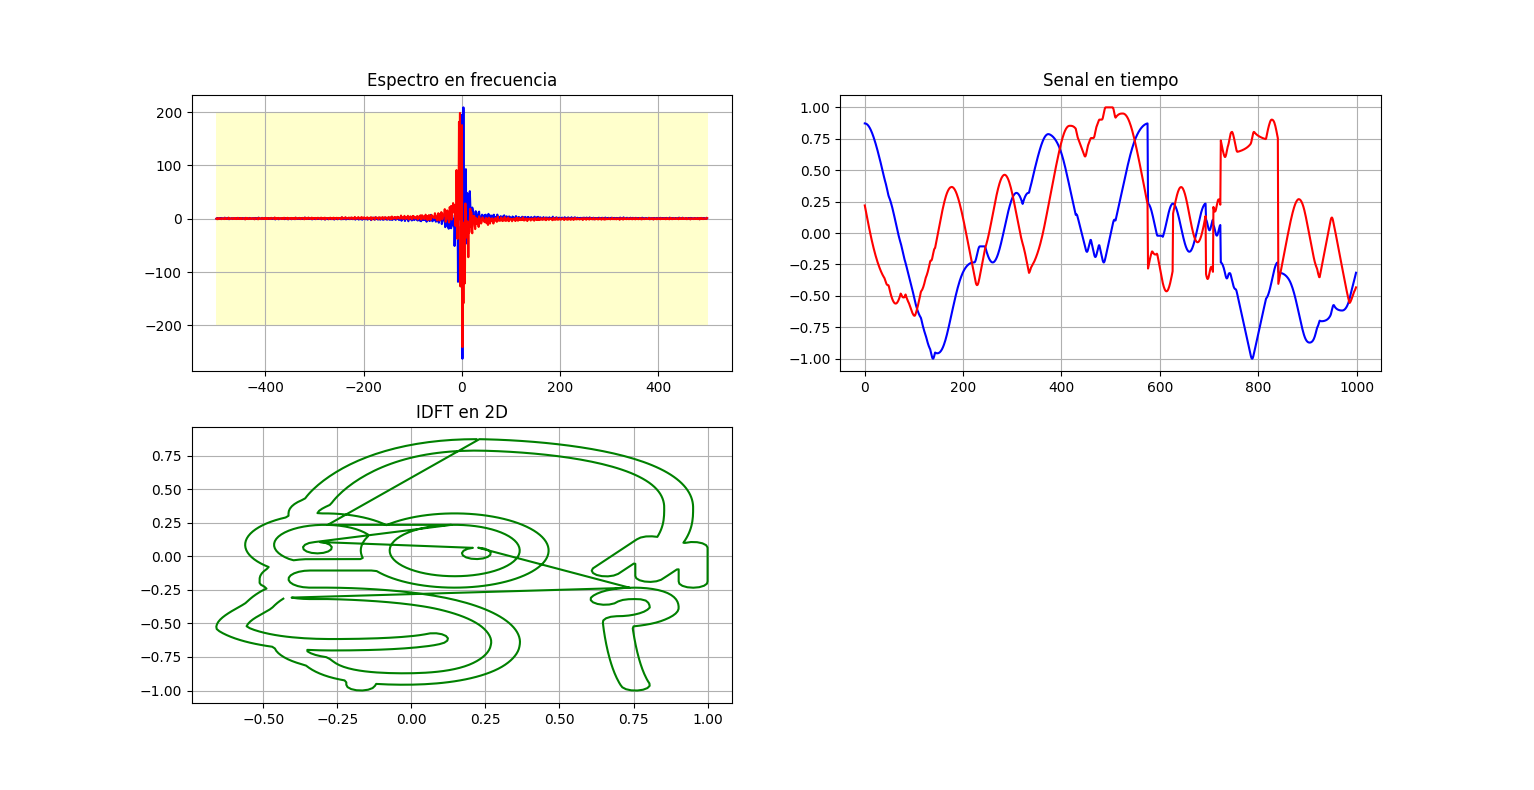
\includegraphics[width=\textwidth]{img/homero.png}
	\caption{Imagen de las señal.}
	\label{fig:ifdt}
\end{figure}

\begin{figure}[htbp]
	\centering
	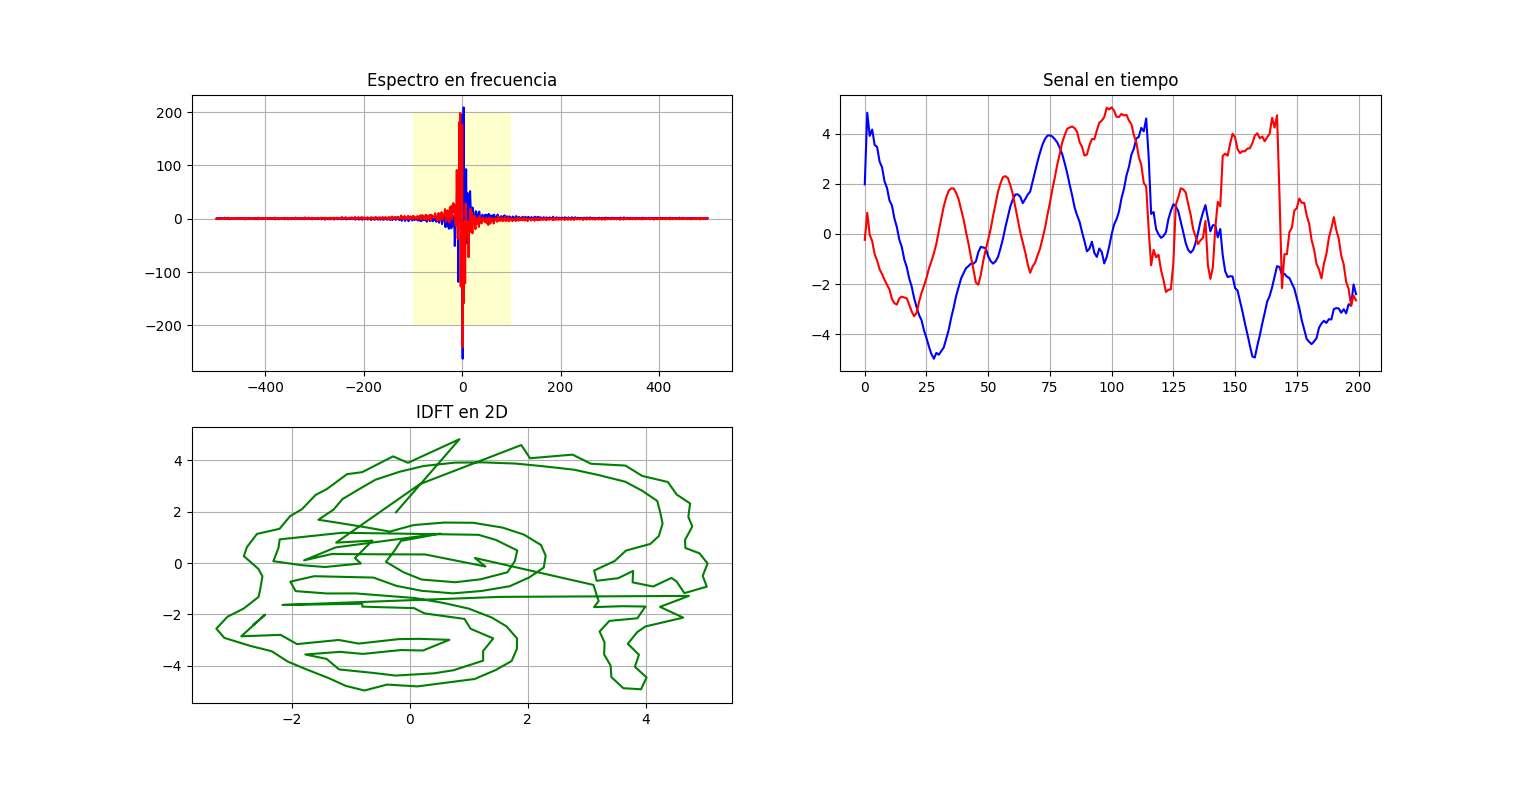
\includegraphics[width=\textwidth]{img/homero200.png}
	\caption{Imagen de las señal con fs de 200 Hz.}
	\label{fig:ifdt}
\end{figure}

\end{document}